\section{Beleuchtung \& Schattierung}

Eigenschaften eines Objektes:
\begin{itemize}
	\item Spiegelung
	\item Glanz / Matt
	\item Transparenz
	\item Glatt / Rau (Oberflächenstruktur) 
	\item Farbe
	\item Struktur / Textur
	\item Brechnung des Lichts
	\item Anisotop (Richtungsabhängig)
\end{itemize}


\subsection{Beleuchtungsmodelle}
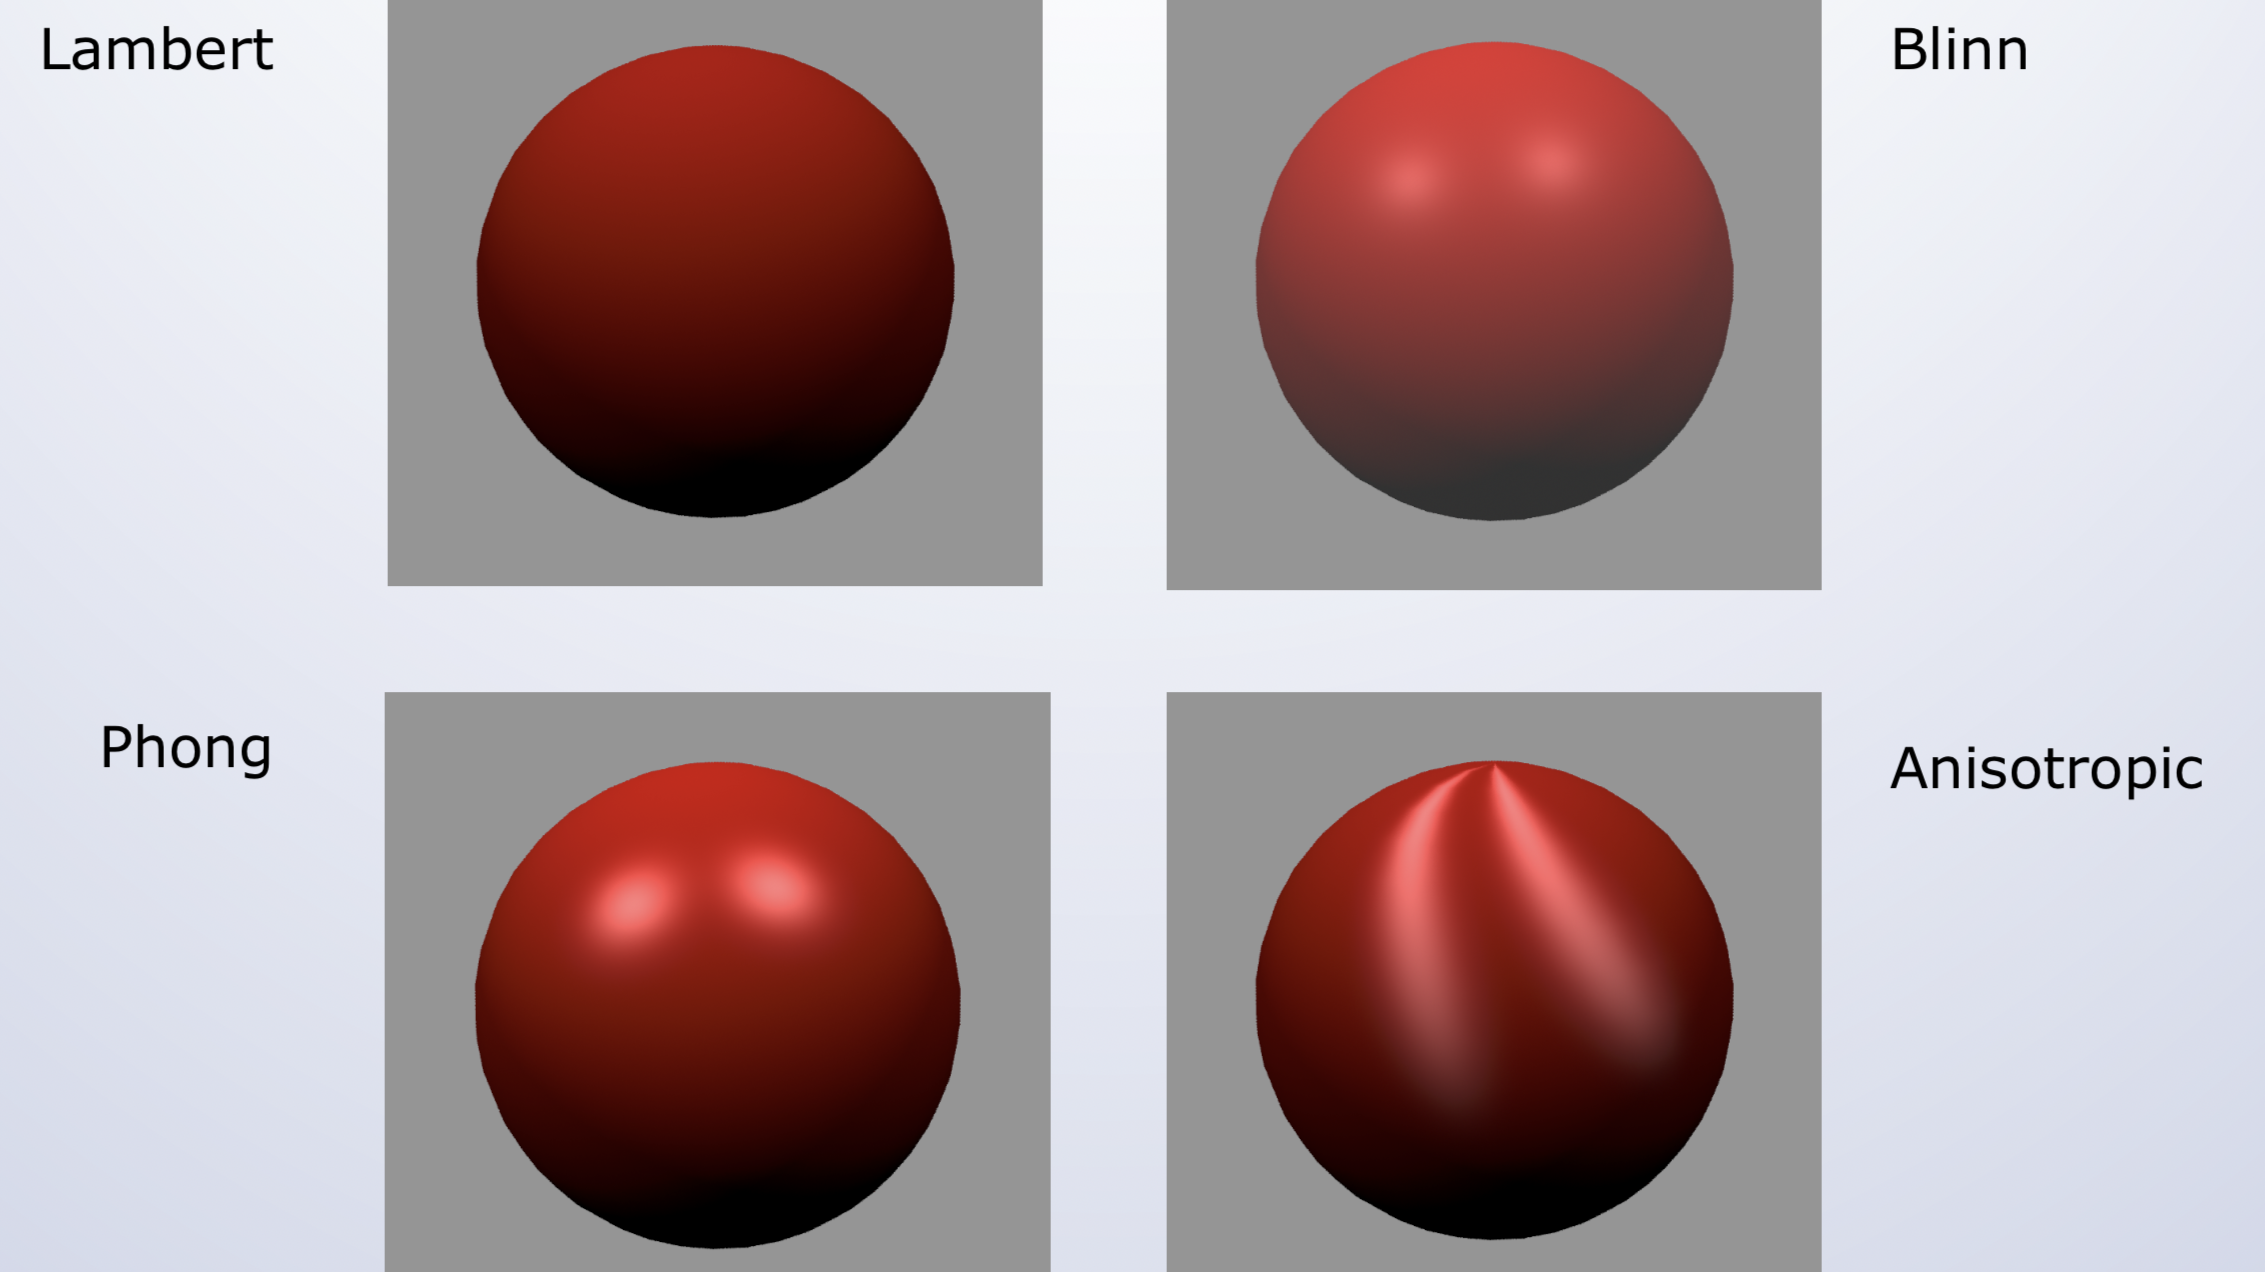
\includegraphics[width=0.45\textwidth]{assets/Beleuchtungsmodelle.png}

TODO Formeln

\subsubsection{Diffuse Reflektion (Lambert Modell)}

\begin{itemize}
	\item Gleichmässige Abstrahlung des Lichts in alle Richtungen
	\item Eigenschaften eines matten, nicht glänzenden Materials
	\item Schiefe Fläche = senkrechte Fläche / cos(a)
	\item reflektierte Intensität = Intensität der Lichtquelle * Reflektierungsfaktor * cosj \\
	cosj = Flächennormale(vektor) * Richtung zur Lichtquelle(vektor) \\
	Reflektierungsfaktor = Farbe des Materials
\end{itemize}

\subsubsection{Spiegelnde Reflektion (Phong Modell)}

\begin{itemize}
	\item Intensität Spiegelung = Intensität der Lichtquelle * Reflektierungsfaktor * cos\textsuperscript{n}(Winkel zwischen Betrachgung \& Reflektionsrichtung) \\
	n = Streuung des Lichts (hohes n -> nimmt schnell ab) \\
	Reflektierungsfaktor = Farbe der Reflektion
\end{itemize}

\subsection{Lichtquellen}

\begin{itemize}
	\item Ambiente Lichtquelle (Licht von überall) 
	\item Direktionale Lichtquelle
	\item Punkt Lichtquelle
	\item Spot Lichtquelle (alles ausserhalb schwarz)
	\item Verteilte Lichtquelle (Licht mit Ausdehnung)
\end{itemize}

\subsection{Schattierung}

\begin{itemize}
	\item Konstanter Schattierung \\
	pro Fläche eine Beleuchtung (Farbe) berechnen

	\item Gouraud Schattierung \\
	Beleuchtung an den Ecken berechnen \\
	dazwischen interpolieren \\
	VertexShader

	\item Phong Schattierung \\
	Beleuchtungsberechnung pro Pixel \\
	FragmentShader
\end{itemize}